%
% riemann.tex
%
% (c) 2017 Prof Dr Andreas Müller, Hochschule Rapperswil
%
\documentclass[tikz]{standalone}
\usepackage{times}
\usepackage{txfonts}
\usepackage{pgfplots}
\usepackage{csvsimple}
\usetikzlibrary{arrows,intersections}
\begin{document}
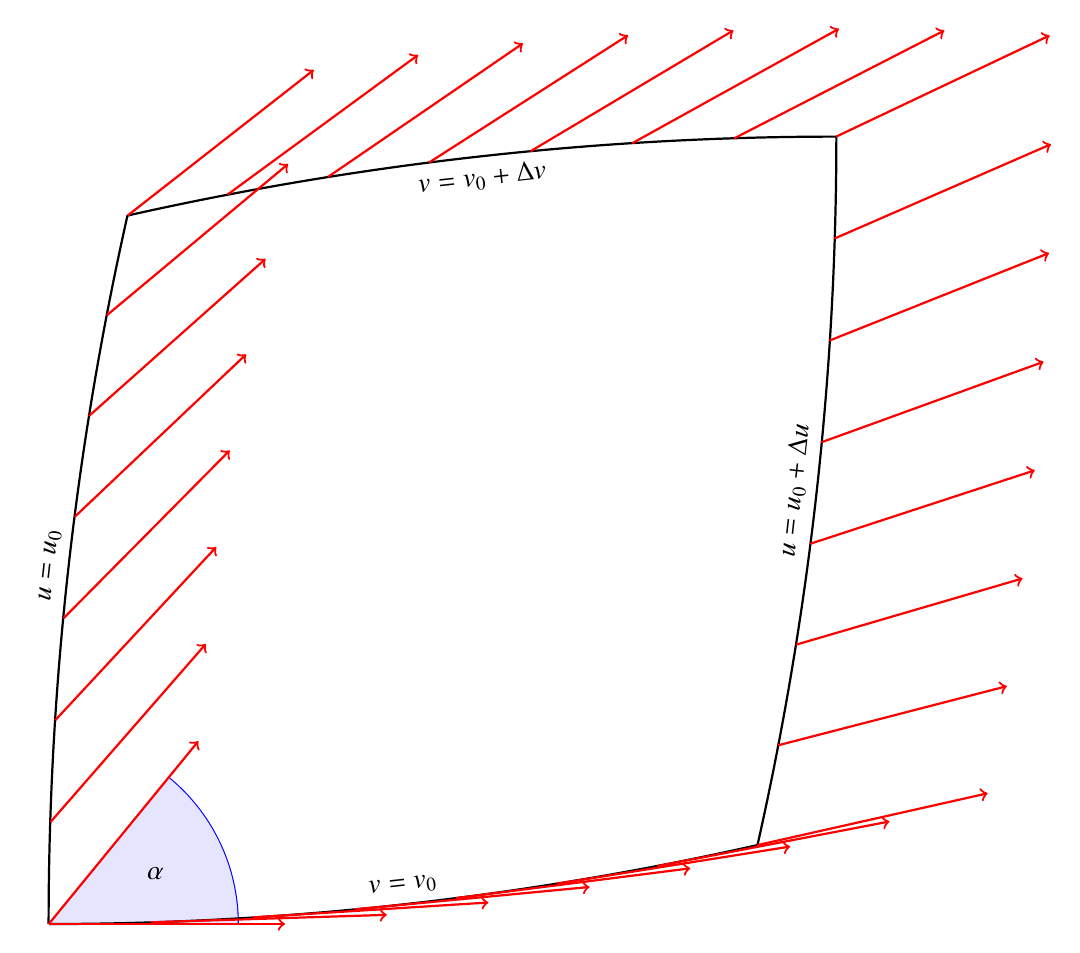
\begin{tikzpicture}[thick,scale=1]
\coordinate (O) at (0,0);

\def\a{5}
\def\b{12}
\def\c{13}

\def\a{12}
\def\b{35}
\def\c{37}

\def\a{9}
\def\b{40}
\def\c{41}

%\def\a{11}
%\def\b{60}
%\def\c{61}

\def\l{3cm}

\coordinate (A) at (0,0);
\coordinate (B) at ({\a},{\c - \b});
\coordinate (C) at ({\a + \c - \b},{\a + \c - \b});
\coordinate (D) at ({\c - \b},{\a});

\coordinate (P) at ({\a + \c - \b},{\a - \b});
\coordinate (Q) at ({\c},0);
\coordinate (R) at (0,{\c});
\coordinate (S) at ({\a - \b},{\a + \c - \b});

\def\ang{atan(\a/\b)}
\def\steps{7}
\def\stept{6}
\def\astep{(\ang / \steps)}

\coordinate (Aa) at ([xshift={\l}]A);
\coordinate (Cc) at ([xshift={cos(2*\ang) * \l},yshift={sin(2*\ang) * \l}]C);
\coordinate (E) at ([xshift={cos(4*\ang) * \l},yshift={sin(4*\ang) * \l}]A);

\coordinate (F) at ([xshift={\l * 0.8}]A);

\draw[blue] (F) arc (0:{4*\ang}:{0.8*\l});

\fill[color=blue!10] (A)--(F) arc (0:{4*\ang}:{0.8*\l})--cycle;

\draw (A) arc (-90:{-90 + \ang}:{\c});
\draw (B) arc ({-\ang}:0:{\c});
\draw (C) arc (90:{90+\ang}:{\c});
\draw (D) arc ({180-\ang}:180:{\c});

%\draw[->,rotate around={10:(0,13)},red]
\foreach \w in {0,...,{\stept}} {
	\draw[->,red] ([rotate around={{(\w*\astep)}:(R)}]A)--
			([rotate around={{(\w*\astep)}:(R)}]Aa);
	\draw[->,red] ([rotate around={{(\w*\astep)}:(P)}]C)--
			([rotate around={{(\w*\astep)}:(P)}]Cc);
}

\foreach \w in {1,...,{\steps}} {
	\draw[->,red] ([rotate around={{-\w*\astep}:(S)}]C)--
			([rotate around={{-\w*\astep}:(S)}]Cc);
	\draw[->,red] ([rotate around={{-\w*\astep}:(Q)}]A)--
			([rotate around={{-\w*\astep}:(Q)}]E);
}

\draw[->,red] (A)--(E);

\node at ({0.5*\l*cos(2*\ang)},{0.5*\l*sin(2*\ang)}) [scale=1] {$\alpha$};

\node at (A) [above,rotate around={{\ang/2}:(R)},scale=1] {$v=v_0$};
\node at (C) [below,rotate around={{\ang/2}:(P)},scale=1] {$v=v_0+\Delta v$};

\coordinate (H) at ({\a - \b},{\a - \b});
\node at (H) [above,rotate around={{90-\ang/2}:(S)},scale=1] {$u=u_0+\Delta u$};

\coordinate (I) at ({\c},{\c});
\node at (I) [above,rotate around={{90-\ang/2}:(Q)},scale=1] {$u=u_0$};

\end{tikzpicture}
\end{document}

